\documentclass[
  digital, %% This option enables the default options for the
           %% digital version of a document. Replace with `printed`
           %% to enable the default options for the printed version
           %% of a document.
  twoside, %% This option enables double-sided typesetting. Use at
           %% least 120 g/m² paper to prevent show-through. Replace
           %% with `oneside` to use one-sided typesetting; use only
           %% if you don’t have access to a double-sided printer,
           %% or if one-sided typesetting is a formal requirement
           %% at your faculty.
  table,   %% This option causes the coloring of tables. Replace
           %% with `notable` to restore plain LaTeX tables.
  nolof,     %% This option prints the List of Figures. Replace with
           %% `nolof` to hide the List of Figures.
  nolot,     %% This option prints the List of Tables. Replace with
           %% `nolot` to hide the List of Tables.
  %% More options are listed in the user guide at
  %% <http://mirrors.ctan.org/macros/latex/contrib/fithesis/guide/mu/fi.pdf>.
]{fithesis3}
%% The following section sets up the locales used in the thesis.
\usepackage[resetfonts]{cmap} %% We need to load the T2A font encoding
\usepackage[T1,T2A]{fontenc}  %% to use the Cyrillic fonts with Russian texts.
\usepackage[
  main=english, %% By using `czech` or `slovak` as the main locale
                %% instead of `english`, you can typeset the thesis
                %% in either Czech or Slovak, respectively.
  english, german, russian, czech, slovak %% The additional keys allow
]{babel}
%% The following section sets up the metadata of the thesis.
\thesissetup{
    date          = \the\year/\the\month/\the\day,
    university    = mu,
    faculty       = fi,
    type          = bc,
    author        = Attila Zsíros,
    gender        = m,
    advisor       = Mgr. Jan Čejka,
    title         = {Using Kalman filters for pose estimation of mobile devices in simulated                     underwater environments},
    TeXtitle      = {Using Kalman filters for pose estimation of mobile devices in simulated                     underwater environments},
    keywords      = {Augmented reality, Extended Kalman filter, iMareCulture, Kalman filter,                     Motion tracking, Odometry, Pose estimation},
    TeXkeywords   = {Augmented reality, Kalman filter, Extended Kalman filter, iMareCulture,                     Motion tracking, Odometry, Pose estimation},
    abstract      = {This is the abstract of my thesis, which can

                     span multiple paragraphs.},
    thanks        = {These are the acknowledgements for my thesis, which can

                     span multiple paragraphs.},
    bib           = bibliography.bib,
}
\usepackage{makeidx}      %% The `makeidx` package contains
\makeindex                %% helper commands for index typesetting.
%% These additional packages are used within the document:
\usepackage{paralist} %% Compact list environments
\usepackage{amsmath}  %% Mathematics
\usepackage{amsthm}
\usepackage{amsfonts}
\usepackage{url}      %% Hyperlinks

\usepackage[textwidth=2.5cm]{todonotes}
\setlength{\marginparwidth}{2.5cm}

\usepackage{siunitx}

\usepackage{markdown} %% Lightweight markup
\usepackage{listings} %% Source code highlighting
\lstset{
  basicstyle      = \ttfamily,%
  identifierstyle = \color{black},%
  keywordstyle    = \color{blue},%
  keywordstyle    = {[2]\color{cyan}},%
  keywordstyle    = {[3]\color{olive}},%
  stringstyle     = \color{teal},%
  commentstyle    = \itshape\color{magenta}}
\usepackage{floatrow} %% Putting captions above tables
\floatsetup[table]{capposition=top}
\begin{document}
\renewcommand{\sectionautorefname}{Section}
\chapter*{Introduction}
\addcontentsline{toc}{chapter}{Introduction}

Augmented reality (AR) is one of the most promising technologies of the present, even though it was grounded already in 1968, when Ivan Sutherland introduced the head-mounted display \cite{68Sutherland}. Since that time, extensive research was conducted on one of the base problems of AR: determining the position and orientation of the device relative to its environment, called the pose estimation problem. Only in recent years, the advances in mobile computing and the release of various AR frameworks, such as ARCore \cite{ARcore}, ARKit \cite{ARkit}, and Vuforia \cite{Vuforia}, allowed delivering a truly seamless AR experience on smartphones. These frameworks are able to leverage the images from the camera and the inertial sensors to produce accurate pose estimates of the device. Hence, the rendered objects appear to coexist seamlessly with the real world. AR has many applications in our lives; for example, in education \cite{ARedu}, healthcare \cite{ARhealth}, or game industry \cite{ARgame}. Another area where AR has the potential to be utilized is the underwater world, which is one of the main aims of the project iMareCulture. It intends to promote the underwater cultural heritage through the use of immersive technologies, so that, for example, tourist scuba divers can explore the archaeological sites \textit{in situ}, with an original reconstruction of the site rendered on the screen of a mobile device.

However, utilizing AR underwater is even nowadays an open problem. The underwater environments often suffer from poor visibility conditions, water turbidity, or no GPS signal, which does not allow the popular AR platforms to perform as accurately as on land. Even though there exist some underwater localization systems, they are expensive, require the use of external equipment, and are too robust for mobile AR.

Within the iMareCulture project, this thesis contributes to the research of underwater AR by analyzing the effect of underwater conditions on the current pose estimation systems. The focus is on marker-based visual-inertial pose tracking systems that use Kalman filtering for sensor fusion. First, a robotic pose estimation system is utilized for the use with smartphone measurements. Second, the pose estimation accuracy in underwater environments is evaluated on various datasets. However, evaluating the experiments directly underwater is difficult due to the absence of ground truth; instead, the underwater conditions are simulated in the controlled environment of a laboratory equipped with a motion capture system. Poor visibility and water turbidity are simulated by post-processing the datasets. Then, the obtained pose estimates are compared to the motion capture measurements, serving as ground truth reference. Finally, conclusions are drawn about the relationship between the simulations and the pose estimation accuracy.

The thesis is structured as follows. The first chapter introduces the background of this thesis, which is the iMareCulture project. The second chapter gives an overview of the pose estimation techniques and discusses their use underwater. The third chapter describes a widely used sensor fusion algorithm, the Kalman filter. The fourth chapter introduces our method of simulating underwater environments. Finally, the fifth chapter describes our experiments and draws conclusions based on the resutls.
\todo[inline]{references}

\chapter{Background}
    The seabed is often called the biggest museum in the world. Throughout the history of human civilizations, entire cities have been flooded, and thousands of ships have sunken to the bottom of the lakes, seas, and oceans. In this subaqueous environment, they have been safely protected for thousands of years. Now they are a part of our cultural heritage in the same way as the heritage on land.
    
    Advances in technology have made the underwater world more accessible and therefore brought these sites within reach. The visitors are offered \textit{in situ} experiences, which include dive trails, submersible tours for non-divers, and underwater museums \cite{unesco_online}.
    
    This thesis is a part of the \textbf{iMare-Culture} project, which focuses on promoting them to the wide public through the use of interactive technologies, virtual reality (VR), augmented reality (AR), and serious games\footnote{A serious game is a game designed for a primary purpose other than pure entertainment.}; all designed by scientists, researchers, archaeologists, and museum experts coming from eight Mediterranean countries. \autoref{fig:baia} shows an example of AR utilization underwater. 
    
    \begin{figure}[h]
        \centering
        \includegraphics[width=.5\textwidth]{img/Background/Baia2.jpg}
        \caption{First pilot test of the underwater AR tablet in Baiae, Italy. AR could be in the future used underwater by tourist scuba divers to explore archaeological sites \textit{in situ} and, for example, observe their original reconstructions on the screen of a mobile device. From iMareCulture \url{https://imareculture.eu}}
        \label{fig:baia}
    \end{figure}

\chapter{Pose estimation for Augmented Reality}
As Azuma defined in 1997, AR systems supplement the real world with virtual (computer-generated) objects that appear to coexist seamlessly with the real world. Besides aligning real and virtual objects with each other, these systems have to be interactive and real time \cite{97azuma}. In contrast with VR, where the user is immersed in a virtual environment, AR allows interaction with virtual objects in a seamless way.

The main AR research topics are Tracking Techniques, Interaction Techniques, Calibration and Registration, AR Applications, and Display Techniques \cite{17ISMAR}. The most popular amongst them are the tracking techniques, since good pose tracking is vital to deliver a seamless AR experience.

The tracking techniques are concerned with determining the pose of the camera, i.e., its position and orientation relative to a reference frame. Despite the enormous progress in this field in the last ten years, it is still challenging to achieve low latency tracking with high precision, accuracy, jitter, and lag in a mobile device. If we compare AR and VR again, but now in terms of tracking requirements, AR pose tracking is more demanding, since errors in registration are easier to detect by the user \cite{93Azuma}.

The tracking problem gets even more complex in underwater environments, where the system has to be waterproof, has to withstand the high pressure of diving depth, cannot rely on GPS, and the captured images suffer from turbidity effects caused by the medium. Furthermore, the amount and cost of sensors packed in smartphones are much more limited than in specialized devices used in, for example, robotics \cite{vi-sensor}. As a consequence, the measurements are noisier and biased. Tracking techniques tackle these problems by integrating several sensors with complementary characteristics into a sensor fusion filter.

This chapter gives an overview of the popular pose estimation techniques and their utilization in the sea.

    \section{Visual tracking}
    Vision-based techniques use computer vision methods to calculate the camera pose relative to real-world objects \cite{99SoYou,02Pinz}. 
    
    They provide high accuracy over a large workspace, as well as low jitter and no drift. The frames are grabbed at rates of 30--60~Hz. 
    
    The general drawbacks include that they require line-of-sight between the camera and the detected target, and that motion blur in the image during drastic motions leads to temporary loss of real-time tracking abilities.
    
    \todo[inline]{Tracking methods detect the distinctive features in the image, some of which may be natural, other artifical. The techniques that rely on artificial features are called marker-based}

        \subsection{Camera calibration}
        When capturing the calibration images, we were following the MATLAB camera calibration workflow\footnote{\url{https://www.mathworks.com/help/vision/ug/single-camera-calibrator-app.html}}. According to this workflow, between 10 and 20 images of the checkerboard pattern should be used to achieve a good camera calibration. In addition, the images should be captured at a distance roughly equal to the camera distance from the objects of interest, without using autofocus or changing the zoom settings between images. Furthermore, since lens distortion increases radially from the center of the image and sometimes is not uniform across the image frame, the images should be taken at different orientations relative to the camera and the pattern must appear close to the edges of the captured images.
        \todo[inline]{... When the image is rectified, the it can be used for marker detection. The targets of the detector are either markers (marker-based tracking) or distinctive features in the image (marker-less tracking). }
        
        \begin{figure}
        \begin{center}
            \begin{minipage}{.29\textwidth}
                \begin{center}
                    \includegraphics[width=.6\textwidth]{img/Markers/AprilTag.png} \\ 
                    \footnotesize(a) AprilTag \cite{AprilTag} \\
                    \vspace{0.6cm}
                    \includegraphics[width=.6\textwidth]{img/Markers/Elipses.png} \\
                    \footnotesize(d) Ellipse \cite{Ellipse} \\
                    \vspace{0.6cm}
                    \includegraphics[width=.6\textwidth]{img/Markers/reacTIV.png} \\
                    \footnotesize(d) reacTIVision \cite{reacTIVision} \\
                \end{center}
            \end{minipage}
            \begin{minipage}{.29\textwidth}
                \begin{center}
                    \includegraphics[width=.6\textwidth]{img/Markers/ARTag.jpg} \\
                    \footnotesize(b) ARTag \cite{ARTag} \\
                    \vspace{0.6cm}
                    \includegraphics[width=.6\textwidth]{img/Markers/CCTag.png} \\
                    \footnotesize(e) CCTag \cite{CCTag} \\
                    \vspace{0.6cm}
                    \includegraphics[width=.6\textwidth]{img/Markers/RUNE.png} \\
                    \footnotesize(e) RUNE-Tag \cite{RUNETag} \\
                \end{center}
            \end{minipage}
            \begin{minipage}{.29\textwidth}
                \begin{center}
                    \includegraphics[width=.6\textwidth]{img/Markers/ARToolKit.pdf} \\
                    \footnotesize(c) ARToolKit \cite{ARToolKit} \\
                    \vspace{0.6cm}
                    \includegraphics[width=.6\textwidth]{img/Markers/Intersense.png} \\
                    \footnotesize(e) Intersence \cite{Intersence} \\
                    \vspace{0.6cm}
                    \includegraphics[width=.6\textwidth]{img/Markers/FourierTag.png} \\
                    \footnotesize(e) Fourier Tag \cite{FourierTag} \\
                \end{center}
            \end{minipage}
        \end{center}
            \caption{Existing fiducial marker designs}
            \label{fig:Markers}
        \end{figure}
        
        \subsection{Marker-based tracking}
        Marker-based tracking methods simplify the problem of detecting 3D objects by detecting only 2D artificial markers that are easy to recognize \cite{19Cejka}. The most dominant technique in marker-based tracking is detecting square markers. They are easy and fast to detect and contain enough information to compute their relative pose to the camera. Examples of some software libraries are ARToolKit \cite{ARToolKit}, ARTag \cite{ARTag}, ARUco \cite{ARUco}, AprilTag \cite{AprilTag}. 
        
        \autoref{fig:Markers} shows that besides square markers, other types of markers are also used in AR \cite{RUNETag, Intersence, reacTIVision, CCTag, FourierTag}. For example, the shape of circular \cite{Intersence} or elliptic markers \cite{Ellipse} provides more information about the position than in the case of square markers. Thus, they can be detected even when they are partially occluded; however, this is paid by higher processing time.
        
        \subsection{Marker-less tracking}
        Instead of detecting artificial markers, marker-less tracking methods detect the distinctive features in the image, such as edges, corners, or textures. The detection algorithms consist of two parts: detection of these features and computation of a descriptor for each feature that can match the features between the frames \cite{19Cejka}. 
        
        The speed and accuracy depend on the complexity of the scene. While simple targets like blobs or corners can be easily identified, cluttered scenes with many objects moving independently are extremely difficult to handle \cite{02Pinz}. This method is also not suitable for texture-less environments. 
        
        Examples of algorithms for natural features detection used in augmented reality are: SIFT \cite{SIFT}, SURF detector \cite{SURF}, and FAST \cite{FAST}. Marker-less tracking is further used in simultaneous localization and mapping (SLAM) solutions described in \autoref{subsec:SLAM} on page~\pageref{subsec:SLAM}.
        
        \subsection{Underwater visual tracking} \label{subsec:underwater_visual}
        Underwater localization from vision is still an open problem, and the state-of-the-art algorithms in visual odometry or SLAM do not give satisfactory results \cite{17Weidner}. Most of the difficulties arise due to visual degradations caused by the medium. The strong light absorption shortens the visual perception to a few meters and makes the presence of an artificial lighting system mandatory when operating in deep waters. The propagation of light is scattered by floating particles, causing turbidity effects on the captured images. The artificial light attracts the animals, and they tend to get in the field of view of the camera, which leads to occlusions in the images.
        
    \section{Inertial tracking}
    Most smartphones contain an Inertial Measurement Unit (IMU) for monitoring the body's movement or orientation in 3D space with respect to the Earth coordinate system. The IMU consists of a triple axis accelerometer and a triple axis gyroscope.
    
    The accelerometer senses the acceleration of the sensor along of each input axis, while the gyroscope measures the angular velocity around each input axis. Together, they form a 6 DoF (Degrees of Freedom) tracking system, providing movement tracking in 3 axes plus rotation in 3 axes (pitch, roll, yaw). Sometimes a third set of sensors, magnetometers, is added for heading reference (the yaw axis), measuring the Earth's magnetic field. However, since they are easily disturbed by any nearby metallic substance, they are often neglected in pose estimation systems \cite{08ISMAR}.
    
    \subsection{MEMS} \label{subsec:MEMS}
    As opposed to the traditional mechanical IMUs, the IMUs in smartphones are based on MEMS (Microelectromechanical systems) technology. On the one hand, this makes them lightweight, compact, power-efficient, and less expensive, thus well suited for mobile computing. On the other hand, due to imperfections of the manufacturing and physical characteristics of the sensors, real IMU measurements are usually affected by random noise and systematic errors, such as the bias (the offset of the sensor measurement from the physical input), inaccurate scale factor (the relation between input and output), axis misalignments, or g-sensitivity \cite{19Xiao, 94Titteron, 03Nassar}. These errors may significantly influence the performance of visual-inertial methods.
    
    The following example illustrates these errors on the accelerometer: The accelerometer measures proper accelerations that are accelerations relative to free fall. For example, if the device is laying flat on the table, the accelerometer should measure an acceleration of $1g \approx \SI{9.81}{\metre\per\square\second}$ away from the center of the Earth. In contrast, when the device is in free fall, it should measure zero. However, due to the bias of \SI{-0.06}{\metre\per\square\second} and random noise of \SI{0.02}{\metre\per\square\second}, the measured acceleration is \SI{9.77}{\metre\per\square\second}.
    
    Thus, the sensor measurements are modeled as follows:
    \begin{align} 
        a_m &= (a - g) + b_a + n_a \\
        w_m &= w + b_\omega + n_\omega
    \end{align}
    where $a_m$ and $w_m$ are the raw measurements of accelerometer and gyroscope, respectively; $a$ and $w$ are linear acceleration and angular velocity of the body frame, $g$ is the gravity vector, $b_a$ and $b_\omega$ are the accelerometer and gyroscope biases, and $n_a$ and $n_\omega$ are the measurement noises. For other IMU measurement models involving scale factors, axis misalignment, g-sensitivity, etc., please refer to \cite{16Rehder}.
    
    \subsection{IMU Calibration}
    IMU calibration is used to identify the value of bias and other intrinsic parameters of sensors for compensating the measurement errors \cite{19Xiao}. It is performed by comparing the raw measurements to some known reference values and minimizing the differences between them. The reference calibration values can be estimated offline or online. 
    
    Offline calibration is relevant in the case of high-performance sensors manufactured precisely or factory calibrated carefully. Such sensors are sold with their own calibration parameters stored into the firmware \cite{14Tedaldi}. 
    However, in consumer electronics, low-cost IMUs are used. The traditional high-precision calibration methods require special external equipment, such as a motion tracking system \cite{04Kim}, which is often time-consuming and more expensive than the IMU itself. Moreover, the intrinsic calibration parameters may vary with mechanical shocks, temperature, and other factors. Treating these parameters as a constant would lead to performance degradation of the inertial tracking system \cite{19Xiao}. For an example of offline accelerometer calibration, please refer to \cite{98Lotters}.
    
    In contrast, online calibration is repeating the calibration process periodically. It is performed real-time and without any external equipment. For example, Xiao et al. \cite{19Xiao} used this method to concurrently perform 3D pose estimation and online IMU calibration based on optimization methods in unknown environments without any external equipment. The pose tracking system used in this thesis also utilizes the online calibration method.
    
    \subsection{Other IMU drawbacks} \label{subsec:IMU_drawbacks}
    Besides bias and gain, another issue, which arises when using IMUs for navigation, is the drift: an ever-increasing difference between where the system thinks it is located and its actual location. Even small errors in measurements lead to large drifts due to the integrating them with respect to time. 
    
    Integrating the acceleration once returns velocity, and integrating the acceleration twice returns position. However, the small errors in the accelerometer measurements grow linearly in velocity and quadratically in position, accumulating the error over time and causing the drift \cite{08Springer}. If the angular velocity measurements from the gyroscope are integrated to obtain the orientation, the errors accumulate similarly. 
    
    Thus, in many attitude estimation solutions, the accelerometer and the gyroscope are fused together to take advantage of their complementary characteristics: the gyroscope is accurate for quick movements in short periods of time, and the accelerometer can determine the gravitation vector in longer periods of time \cite{99Luinge}. The sensor fusion allows determining the pitch and roll axes, as well as achieving better results than using any of the sensors separately.

    \section{Hybrid tracking}
    As seen in the previous section, the sensor fusion compensates for the respective drawbacks of the accelerometers and the gyroscopes, exhibiting the virtues of both technologies. Hybrid tracking may combine not only the inertial, but many other types of sensors \cite{99SoYou}. Visual-inertial tracking takes advantage of the complementary properties of visual and inertial sensors \cite{16Palonen}. 
    
    On the one hand, the drawbacks of vision tracking, i.e., the low-frequency, line-of-sight requirement, or motion blur, are compensated by the advantages of the IMU, i.e., the high-frequency measurements from the IMU, occlusion immunity, and high accuracy in cases of rapid directional changes or high rotational speed.
    
    On the other hand, the inertial navigation systems are not accurate in slow rotational and translational motions due to bias and drift which is compensated by the high accuracy of the optical tracking system.
    
    Several approaches are addressing the visual-inertial estimation problem. Leutenegger \cite{15Leutenegger} separates them in two ways. First, the methods can be divided into batch nonlinear optimization methods and recursive filtering methods. Second, the two other categories of approaches found in the literature are described in \cite{15Leutenegger} as follows:
    \begin{description}
        \item [loosely coupled systems] they independently estimate the pose by a vision-only algorithm and fuse IMU measurements only in a separate estimation step, limiting computational complexity;
        \item [tightly coupled approaches] they, in contrast, include both the measurements from the IMU and the camera into a common problem where all states are jointly estimated, thus considering all correlations amongst them.
    \end{description}
    In this thesis, the tracking system is based on the recursive filtering of the extended Kalman filter, and the tightly coupled approach, which proved to be essential for any high-precision visual-inertial navigation system, and is implemented in most high-accuracy visual-inertial systems estimators \cite{13Leutenegger}.
    
    \subsection{SLAM} \label{subsec:SLAM}
    Hybrid tracking approaches are often combined with simultaneous localization and mapping (SLAM). SLAM is the computational problem of building a map of an unknown environment and, at the same time, using this map to compute the pose of the tracking device \cite{SLAMII}. It is a marker-less technology, i.e., no markers or image targets are necessary to place in the environment. The map is created by obtaining spatial data of the environment, such as 3D point clouds. 
    
    Mapping and tracking simultaneously have high computational demands on the device, which is also a reason why SLAM solutions were initially employed in systems with specialized equipment, for example, in robotics, self-driving cars, or unmanned aerial vehicles. However, thanks to the advances in computer vision, performance, and sensory navigation of mobile devices in the past decade, smartphones are powerful enough to run AR applications that use SLAM. For general concepts of existing mobile SLAM techniques, please refer to \cite{17Taketomi} and for a survey of 23 chosen methods to \cite{16Younes}.

    Many commercial AR software development kits (SDKs) are based on SLAM due to no need for placing tracking elements in the environment, and the high computing power of today's smartphones. The most powerful and popular SDKs are ARCore (Google) \cite{ARcore}, ARKit (Apple) \cite{ARkit}, and Vuforia (PTC) \cite{Vuforia}. They offer native application programming interfaces (API) for motion tracking, environmental understanding, and light estimation to simplify the task of building an AR application. The developer can make use of the detection of horizontal surfaces, as well as point cloud anchors or lighting of virtual objects matches the surroundings to make their appearance more realistic. Amin and Govilkar \cite{Comparative} give a comparative study of AR SDKs.

    \section{Underwater tracking}
    \label{sec:underwater_pose_estimation}
    In the sea, the number of requirements for an AR system is higher than on land. For example, GPS cannot be used for localization \cite{18Ferrera}, which leads to the use of advanced sensors, such as sonars, acoustic positioning systems, or Doppler velocity loggers (DVLs); however, these sensors are not suitable for mobile AR.
    
    Furthermore, the system has to be waterproof and has to withstand the high pressure of diving depth \cite{18Ferrera}. Thus, the solutions use expensive, robust systems, such as remotely operated vehicles (ROVs) and autonomous underwater vehicles (AUVs).
    
    Some solutions found in the literature rely on IMUs, pressure sensors, and DVLs \cite{14Paull}, which, as discussed in \autoref{subsec:IMU_drawbacks}, leads to unavoidable drift over time due to measurement noise. The drift is constrained using complementary sensors such as cameras or acoustic positioning systems. 
    
    However, at close-range, acoustic systems do not provide accurate enough localization information, whereas visual sensing can be highly effective \cite{18Palomeras}. Nevertheless, as discussed in \autoref{subsec:underwater_visual}, the captured images are degraded by turbidity. Furthermore, the information delivered by sonar is not as rich as optical images \cite{15BoninFont}, and remains very challenging to analyze.
    
\chapter{Kalman filtering}
Filters are used to continuously estimate the state of the system, given noisy sensor measurements. The system's state can be formed by, for example, position, velocity, or orientation of the system. Motion models describe how the system's state changes over time. The filter's task is to fuse the measurements from the sensors and the information from the motion model in the best possible way to calculate the new state estimate \cite{17Fahreus}. 

The Kalman filter happens to perform the filtering in a statistically optimal way. It was introduced in 1960 by R. E. Kálmán in his famous paper \cite{60Kalman}, describing a recursive solution to the discrete data linear filtering problem. Probably the most famous early use of the Kalman filter was in the Apollo 11 Guidance Computer that helped Neil Armstrong to go to the Moon and back \cite{Apollo}. Since that time, it has become extensively researched and applied in navigation systems, robotics, or computer vision, and today, it can be found in every smartphone.

There are many reasons why the Kalman filter is still so popular
\cite{95Intro,09Pose}: 
\begin{itemize}
    \item It is light on memory --- in contrast to batch estimation techniques (e.g., the Wiener filter \cite{Wiener}), which operates on \textit{all} of the data \textit{directly} for each estimate, the Kalman filter is a recursive algorithm and does not need to keep any history of measurements and/or estimates.
    \item It is fast --- due to its low computational cost, it is well suited for real-time problems and embedded systems.
    \item It can estimate a hidden system state --- when the state is not directly measurable, the Kalman filter combines the measurements from multiple sensors to incorporate the missing data and make the state globally observable.
    \item It can handle unsynchronized measurements --- convenient for fusing low-frequency camera images with high-frequency IMU measurements.
\end{itemize}

\section{Dynamical model}
In order to use a Kalman filter to remove noise from a signal, the process that we are measuring must be able to be described by a linear system. At each (discrete) time increment, the new state is generated by applying a linear operator to the previous state, optional control inputs on the system, and adding some noise to cope with changes in the state that are not modeled, according to

\begin{equation} \label{eq:KFlinState}
    x_k = A x_{k-1} + B u_{k-1} + w_{k-1},
\end{equation}

and a new measurement is represented by

\begin{equation} \label{eq:KFlinMeas}
    z_k = H x_k + v_k,
\end{equation}

where
\begin{itemize}
    \item $x_k$ is the state vector at time $k$;
    \item $A$ is the state transition matrix which relates the previous time step $k-1$ to the state at the current step $k$;
    \item $u_{k}$ is the control input vector at time $k$;
    \item $B$ is the control input matrix which relates the control input $u$ to the state $x$;
    \item $w_k$ is the process noise which is assumed to be drawn from a zero mean multivariate normal distribution, $\mathcal{N}$, with covariance $Q_k: w_k \sim \mathcal{N}(0,Q_k)$;
    \item $z_k$ is the measurement vector at time $k$;
    \item $H$ is the transformation matrix that maps the state vector into the measurement domain;
    \item $v_k$ is the measurement noise which is, similarly to $w_k$, assumed to be drawn from a zero mean multivariate normal distribution, $\mathcal{N}$, with covariance 
    $R_k: v_k \sim \mathcal{N}(0,R_k)$. However, it is assumed that $v_k$ and $w_k$ are mutually independent to apply this model in the KF.
\end{itemize}

In pose estimation systems, the state vector usually contains the position, velocity, and orientation of the device. Also, the state often contains the sensors biases estimated online, as described in \autoref{subsec:MEMS}. The measurements are represented by the images from the camera and the inertial sensor readings.

\section{Algorithm}
The Kalman filter combines the prediction and the measurement to find the optimal state estimate in the presence of process and measurement noise. It operates recursively in a cycle: it first \textbf{predicts} an \textit{a~priori} state estimate $\hat{x}_k^-$ based on the dynamic model; and then it receives a noisy measurements $z_k$ from the sensor and uses the difference between the $\hat{x}_k^-$ and $z_k$ as a feedback to optimally \textbf{update} the \textit{a priori} state estimate into an \textit{a~posteriori} state estimate $\hat{x}_k$ \cite{95Intro}.

\begin{figure}[h]
    \centering
    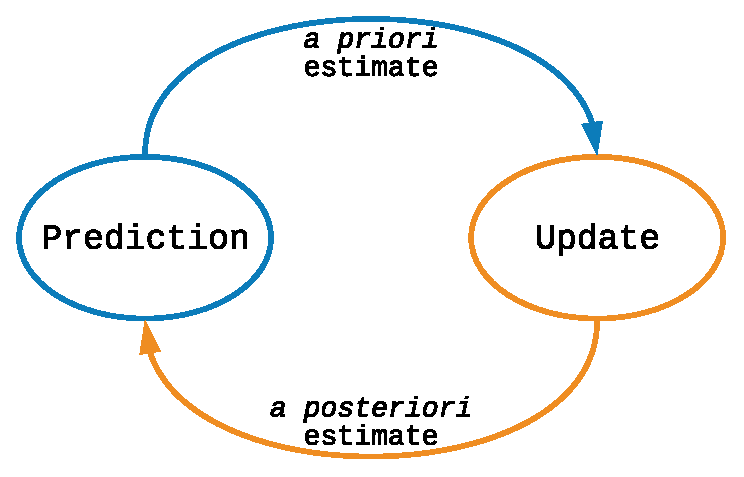
\includegraphics[width=.65\textwidth]{img/KF/Cycle.eps}
    \caption{The ongoing Kalman filter cycle. The prediction stage projects the current state estimate ahead in time forming the \textit{a~priori} state estimate, which is then improved by the measurements in the update stage to form the \textit{a~posteriori} state estimate.}
    \label{fig:KFcycle}
\end{figure}

Since the Kalman filter takes into account also the noises, the state of the filter is represented not only by the (\textit{a posteriori}) state estimate $\hat{x}_k$, but also by its corresponding (\textit{a posteriori}) error covariance matrix $P_k$, which holds the estimated accuracy of the state estimate such that
\begin{equation}
    P_k = E[(x_k - \hat{x}_k) (x_k - \hat{x}_k)^T].
\end{equation}

Here are presented the equations used in the two stages of the Kalman filter.
\begin{enumerate}
    \item Prediction:
        \begin{equation}
            \hat{x}_k^- = A \hat{x}_{k-1} + B u_{k-1}
        \end{equation}
        \begin{equation} \label{eq:KFprocessNoise}
            P_k^- = A P_{k-1}A^T + Q_k
        \end{equation}
        
        \begin{itemize}
            \item $\hat{x}_k^-$ is the predicted (\textit{a priori}) state estimate;
            \item $P_k^-$ is the predicted (\textit{a priori}) estimate error covariance.
        \end{itemize}
        
        The prediction stage projects forward in time, estimating the current state and error covariance to obtain the a priori estimates.
    \item Update:
        \begin{equation} \label{eq:KFkalmanGain}
            K_k = P_k^- H^T (H P_k^- H^T + R_k)^{-1}
        \end{equation}
        \begin{equation} \label{eq:KFweighted_avg}
            \hat{x}_k = \hat{x}_k^- + K_k (z_k - H \hat{x}_k^-)
        \end{equation}
        \begin{equation} \label{eq:KFprocessNoisePost}
            P_k = (I - K_k H) P_k^-
        \end{equation}
        \begin{itemize}
            \item $K_k$ is the Kalman gain at time $k$;
            \item $\hat{x}_k^-$ is the updated (\textit{a~posteriori}) state estimate.
        \end{itemize}
        The update stage incorporates new measurements into the \textit{a~priori} estimates to obtain an improved \textit{a posteriori} estimate.
        
        Notice that the \textit{a~posteriori} state estimate $\hat{x}_k$ in \ref{eq:KFweighted_avg} is obtained as a \textbf{weighted average} between the \textit{a~priori} state estimate $\hat{x}_k^-$ and the measurement residual. The purpose of the weights is that they decide based, which of either the estimate or measurement to ``trust more'' \cite{KalmanWiki}. The Kalman gain is computed based on their uncertainties, so values with better (i.e., smaller) estimated uncertainty are trusted more. Hence, if the prediction is accurate, the Kalman gain cancels out the effect of new measurements, and vice versa.
\end{enumerate}

This process is repeated at every time step, with the new estimate and its covariance informing the prediction used in the following iteration. This means that the Kalman filter works recursively and requires only the last ``best guess'', rather than the entire history, of a system's state to calculate a new state. \todo{Just wiki, rewrite}

\subsection{Parameters} \label{subsec:KFparams}
Since the filtering process starts with an initial state defined by the user, the accuracy of this state can influence the performance of the Kalman filter. Determining the values in the measurement noise covariance matrix $R$ is usually possible and practical because we use the measurement device and are able to get the measurement noise by a calibration routine \cite{95Intro}. On the other hand, finding the process noise covarinace matrix $Q$ is usually more difficult because we are often estimating a process that is not directly observable. Thus, it is often tuned by trial and error; however, as Welch and Bishop state \cite{95Intro}: ``In either case, whether or not we have a rational basis for choosing the parameters, often times superior filter performance (statistically speaking) can be obtained by tuning the filter parameters $Q$ and $R$.''

\section{Non-linear systems}
The presented basic for of the Kalman filter is limited to linear systems. However, many systems used in practice are non-linear and some of the most interesting and successful applications of Kalman filtering have been in such situations. This section briefly presents the two most popular non-linear Kalman filters: the Extended Kalman filter and the Unscented Kalman filter.

\subsection{Extended Kalman filter}
The Extended Kalman filter (EKF) can contain \textit{non-linear} functions in the state transition and measurement models, but these functions have to be of differentiable type. 
The system dynamics is then modeled as follows

\begin{equation}
    x_k = f(x_{k-1}, u_{k}) + w_{k},
\end{equation}

and a new measurement is represented by

\begin{equation}
    z_k = h(x_k) + v_k,
\end{equation}

In this case, $f$ and $h$ are \textit{non-linear} functions. Hence, the covariances cannot be obtained as in (\ref{eq:KFprocessNoise}), (\ref{eq:KFkalmanGain}), and (\ref{eq:KFprocessNoisePost}). Therefore, the EKF linearizes about the mean of the current estimate and covariance, by computing the following Jacobians\footnote{The Jacobian matrix is a matrix of first-order partial derivatives.}

\begin{equation}
    F_k=\left.\frac{\partial f}{\partial x}\right|_{\hat{x}_{k-1}^-, \hat{u}_k}
\end{equation}
\begin{equation}
    H_k=\left.\frac{\partial h}{\partial x}\right|_{\hat{x}_{k-1}}.
\end{equation}

The predict and update equations are as follows
\begin{enumerate}
    \item Prediction:
        \begin{equation}
            \hat{x}_k^- = f(x_{k-1}, u_{k})
        \end{equation}
        \begin{equation} \label{eq:EKFprocessNoise}
            P_k^- = F_k P_{k-1} F_k^T + Q_k
        \end{equation}
        
    \item Update:
        \begin{equation} \label{eq:EKFkalmanGain}
            K_k = P_k^- H_k^T (H_k P_k^- H_k^T + R_k)^{-1}
        \end{equation}
        \begin{equation} \label{eq:EKFweighted_avg}
            \hat{x}_k = \hat{x}_k^- + K_k (z_k - H_k \hat{x}_k^-)
        \end{equation}
        \begin{equation} \label{eq:EKFprocessNoisePost}
            P_k = (I - K_k H_k) P_k^-.
        \end{equation}
\end{enumerate}

The drawbacks of the EKF include that it requires complicated derivatives if done analytically, or is computationally costly if done numerically. Also, due to linearization, the functions have to be differentiable; or, even when a function differentiable but highly non-linear, the EKF performance is poor \cite{UKF}.

\subsection{Unscented Kalman filter}
The unscented Kalman filter (UKF) \cite{UKF} does not solve the non-lineary by linearization, but by a deterministic sampling techcnique, called the unscented transformation. It selects a minimal set of sample points, called sigma points, so that that their mean and covariance is the same as the normal distribution. The sigma points are then fed though the non-linear functions, from which a new mean and covariance estimate are then formed.

However, as Caarls concludes \cite{09Pose}, ``the UKF implementation is more time consuming because instead of one non-linear transformation in the EKF, all sigma points are subject to the same non-linear transformation.'' LaVoila \cite{lavoila} aggrees by showing that the EKF is more suitable for VR orientation tracking than the UKF.
\todo[inline]{shorten}


\chapter{Localization in a simulated underwater environment}
The goal of this thesis is to choose a mobile, fiducial based, visual-inertial pose tracking system, and to evaluate its performance in underwater conditions. To be able to assess the tracking precision, the pose estimates have to be compared to ground truth.

For position and orientation tracking, the ground truth is typically represented by an external motion capture system with submillimeter accuracy \cite{15Neunert}. However, this system can only be installed in a controlled environment of a laboratory and cannot be used in the sea. Thus, the experiments in this thesis are conducted in the laboratory equipped with a motion capture system, and the underwater conditions are simulated by post-processing the marker detection results.

\autoref{sec:pose_system} introduces the chosen underwater localization method for this thesis, \autoref{sec:simulating} describes the poor visibility simulation methods used in the experiments, and \autoref{sec:evaluation} describes the evaluation method for pose estimation accuracy.

\section{Pose estimation system} \label{sec:pose_system}
When choosing a suitable solution for underwater localization in the context of this thesis, various constraints have to be taken into account. As discussed in \ref{sec:underwater_pose_estimation}, some sensors, for example, GPS or magnetometers, are not suitable for underwater use, which already discards a large number of implemented localization systems found in the literature. In addition, even though many underwater localization systems rely on external equipment, such as acoustic positioning systems \cite{14Paull}, our system should use only square fiducial markers.

    \subsection{RCARS}
    Although we did not find any mobile pose tracking system customized for underwater use at the time of our related work research, we found a suitable open source solution from the field of robotics. 
    
    \textbf{RCARS} (Robot-Centric Absolute Reference System) is a fiducial-based, visual-inertial EKF-SLAM pose estimation system,  introduced by Neunert et al. in 2016 \cite{15Neunert}. As the authors claim, coupling SLAM and fiducial based estimation resulted in a leaner estimation and smaller map sizes, which makes the system more lightweight. Moreover, they state that the system is robust against fast motions and provides accurate estimates even in changing lighting conditions.

    \begin{figure}
        \centering
        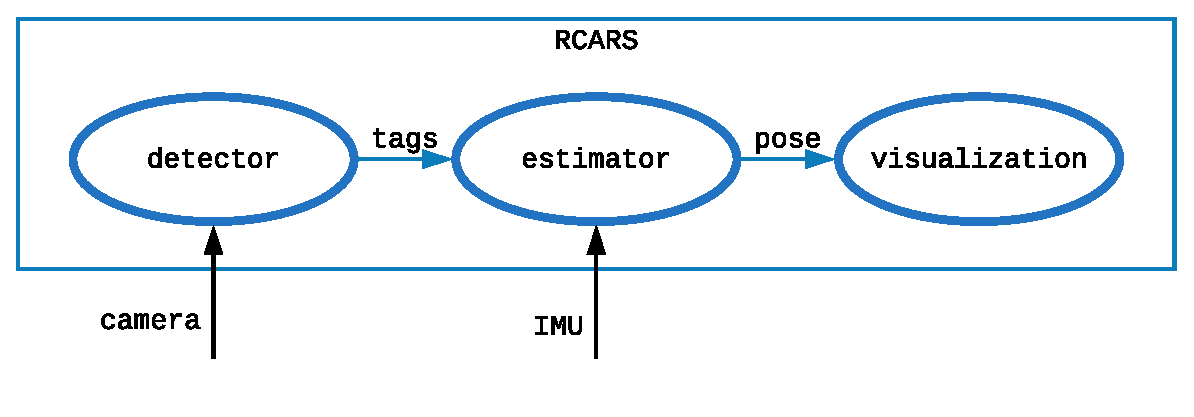
\includegraphics[width=\textwidth]{img/RCARS/RCARS-nodes.eps}
        \caption{RCARS nodes and topics exchanged between them. The detector finds the tags in the images, the estimator calculates the device pose, and the visualization node shows the results in a 3D workspace.}
        \label{fig:RCARSNodes}
    \end{figure}

    \subsection{ROS}
    RCARS is built on the Robot Operating Syste (ROS) software interface. ROS\footnote{\url{https://www.ros.org/}} is an open-source, robotics middleware for creating robot applications. It provides services like hardware abstraction, device drivers, libraries, visualizers, message-passing, or package management. 
    
    ROS-based processes are represented as \textit{nodes} in a graph architecture, connected by edges called \textit{topics}. Topics are buses over which nodes send and receive messages. To send a message, a node must \textit{publish} to a topic, while to receive messages it must \textit{subscribe}. The types of messages passed on a topic vary widely and can be user-defined. The content of these messages can be, for example, sensor data, images, motor control commands, state information, or actuator commands.
    
    \subsection{RCARS packages}
    The RCARS the software structure\footnote{\url{https://bitbucket.org/adrlab/rcars/wiki/Software_Structure}} is depicted in \autoref{fig:RCARSNodes}. RCARS operates on three nodes --- the estimator, the detector, and the visualizer --- and the topics passed between them are, for example, the image, the detected tags, or the pose estimates.

    The detector detects markers in the received undistorted images and publishes marker information, such as the marker id, the marker pose with respect to camera, or the locations of its four corners in the image coordinates. 
    
    \todo{Put AprilTags also here?}
    RCARS uses AprilTags as markers, shown in \autoref{fig:Markers} (a) on page~\pageref{fig:Markers}, which are 2-dimensional, square printable markers with a unique identification number. As a result, they can be robustly tracked and estimated in the EKF. As Neunert et al. reason, AprilTags are used in RCARS due to their high accuracy and the numerous available detector implementations in C/C++. They also state that with AprilTags, high accuracy tracking is achievable even with very few tags, resulting in lower computational demands.

    The Kalman filtering itself is realized by the estimator, which subscribes to the detected markers and the inertial measurements, and outputs the pose estimates of the device, as well as the extrinsic calibration parameters between the IMU and the camera. 
 
    The visualizer uses the  RViz\footnote{\url{http://wiki.ros.org/rviz}} tool for a 3D visualization of the workspace, as well as an image preview. As seen in \autoref{fig:rviz}, the image preview shows the tag corner detections and their corresponding estimations separately. The RViz tool is useful for analyzing the estimation process and identifying the cases when outliers occur.
    
    \begin{figure}
        \centering
        \includegraphics[width=\textwidth]{img/RCARS/rviz3.png}
        \caption{RViz provides a 3D visualization of the workspace, as well as image previews with tag corner detections.}
        \label{fig:rviz}
    \end{figure}
    
    \section{Utilizing RCARS}
    The drawback of RCARS is that it runs only on a computer. Thus, the pose estimation cannot be realized online on the Android smartphone used in this thesis, which leads to a series of steps that need to be  taken in order to obtain the pose estimates from RCARS. This workflow is depicted in \autoref{fig:workflow_pose}.
    
    \begin{figure}
        \centering
        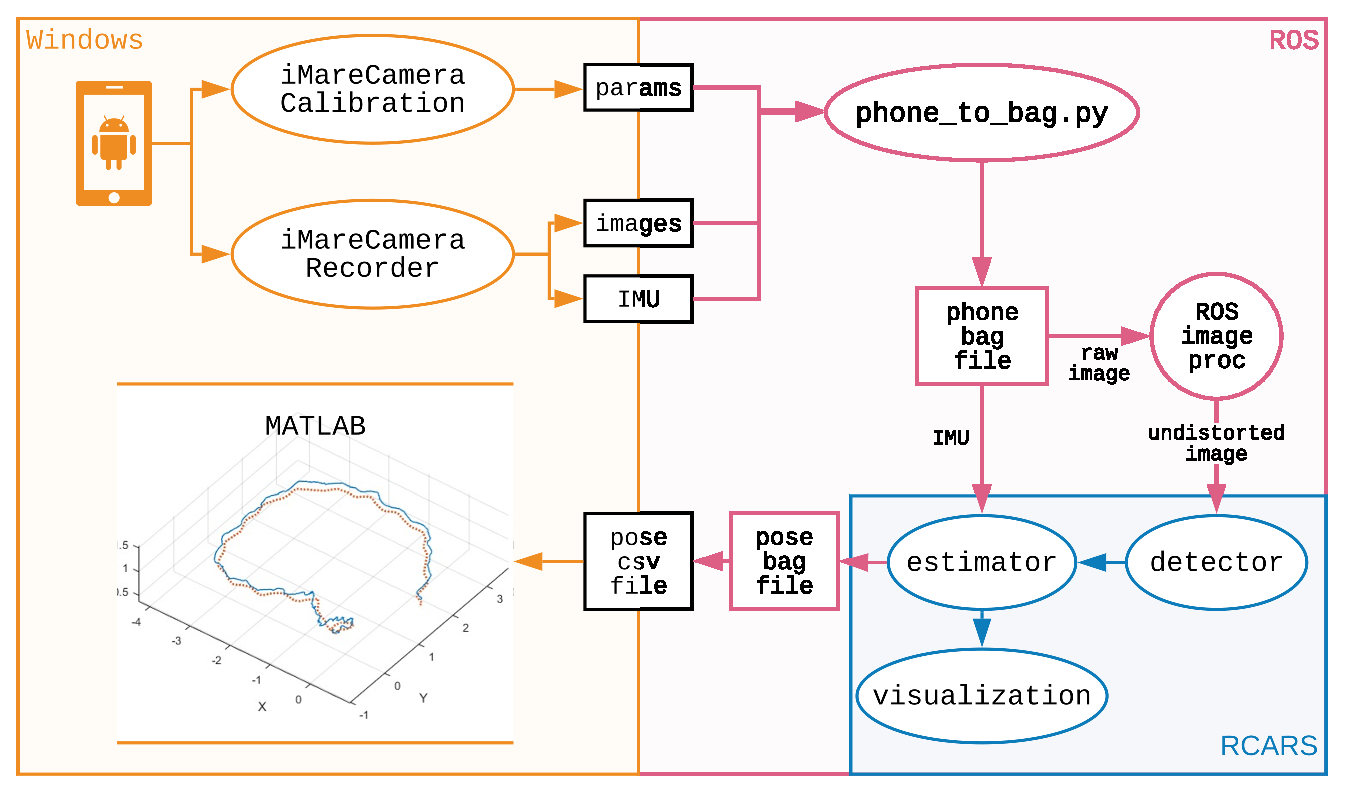
\includegraphics[width=\textwidth]{img/RCARS/workflow_pose.eps}
        \caption{Our pose estimation workflow. First, the smartphone recordings are converted into a bag file. Second, RCARS is run on undistorted images. Third, RCARS outputs the pose estimate that can be visualized or saved for evaluation.}
        \label{fig:workflow_pose}
    \end{figure}
    
    \subsection{Input data} \label{subsec:input_data}
    First, the measurements from the smartphone have to be set as input for RCARS. ROS provides packages\footnote{\url{http://wiki.ros.org/rosserial}} for communication with the serial ports of electronic devices connected to the computer, allowing live sending of data to ROS; however, these packages are built mainly for microcontrollers such as Arduino. Although there is also a driver\footnote{\url{http://wiki.ros.org/android_sensors_driver}} for a  wireless communication with Android devices, it supports only sending GPS and IMU measurements, not the camera images that are needed here.

    Therefore, in our experiment, we first need to record the datasets and then convert the image and the IMU measurements into a proper input format to allow sending them in the ROS ecosystem.
    
    The recording and camera calibration is realized by the iMareCameraRecorder and the iMareCameraCalibration applications developed by Jan Čejka for the AR systems research within the project iMareCulture. The iMareCameraRecorder allows storing uncompressed, time-stamped images and IMU measurements. The iMareCameraCalibration uses the OpenCV algorithm\footnote{\url{https://docs.opencv.org/2.4/modules/calib3d/doc/camera_calibration_and_3d_reconstruction.html}} that calculates both the camera matrix and the radial and tangential distortion coefficients from a chessboard pattern.

    To run RCARS on our measurements, we save them into a \textit{bag}\footnote{\url{http://wiki.ros.org/Bags}} file as ROS \textit{messages}. The bag is a file format for storing ROS message data. The conversion is realized by the \texttt{phone\_to\_bag.py} Python script that uses the \textit{rosbag} Python API\footnote{\url{http://wiki.ros.org/rosbag/Code\%20API\#py_api}} to write into bag files. The messages are stored in a new bag file in the following topics:
    \begin{description}
        \item [\texttt{camera\_info}] holds the camera metadata, such as the intrinsic calibration parameters or the image resolution;
        \item [\texttt{image\_raw}] holds the raw camera images;
        \item [\texttt{imu}] holds the accelerometer and gyroscope measurements.
    \end{description}
	
    The script synchronizes the IMU with the images based on their timestamps. Note that RCARS allows using only one sampling frequency for the IMU measurements. For example, in the case of the iMareCameraRecorder, even though it records the accelerometer at 400Hz and the gyroscope at 200Hz, the accelerometer had to be downsampled to 200Hz to match the frequency of the gyroscope. In addition, we use the \textit{rosbag} tools\footnote{\url{http://wiki.ros.org/rosbag}} for recording and playing back bag files.

    When the bag files are prepared, we play them with rosbag. When the bag file is being played, it appears to RCARS as if there was a live stream of data from a device, which finally allows us to run RCARS on our data.
    
    \subsection{Detection}
    As shown in our workflow in \autoref{fig:workflow_pose} on page \pageref{fig:workflow_pose}, the bag file publishes the raw images and the intrinsic camera calibration parameters to the integrated ROS image processing node\footnote{\url{http://wiki.ros.org/image_proc}} that undistorts them. The detector can then use these images to detect the AprilTags, and then publish their relative poses to the camera, as well as their corner locations.

    \subsection{Estimation}
    The estimator node subscribes to the tag corner detections from the detector and the IMU measurements from the source bag file. However, before running the estimation, we have to configure the EKF parameters stored in the \texttt{EKFsettings.info}\footnote{\url{https://bitbucket.org/adrlab/rcars/wiki/Configuration}} configuration file. As discussed on page \pageref{subsec:KFparams}, configuring the EKF is not trivial, hence we left most of the parameters on default values.
    
    However, there are some parameters that cannot be left on default, because we are using a different device than the authors:
    \begin{description}
        \item [\texttt{Extrinsic calibration}] The extrinsic calibration between the IMU and the camera.
        \item [\texttt{PixelStd}] The squared pixel standard deviation of the tag corner detection results.
        \item [\texttt{MahalanobisTh}] The Mahalonobis threshold distance\footnote{\url{https://en.wikipedia.org/wiki/Mahalanobis_distance}} defining when the marker is considered an outlier.
    \end{description}
	
    Note that enough time should be devoted to determining the correct values for the device, because they are critical for the estimator to work correctly. Also, Neunert et al. \cite{15Neunert} use is the specialized Visual-Inertial (VI-) Sensor\footnote{\url{http://wiki.ros.org/vi_sensor/}} that provides fully time-synchronized and factory calibrated IMU- and stereo-camera data stream. Therefore, we do not expect from a smartphone to perform with such accuracy and robustness in our experiments as the authors achieved.
    
    The estimator then publishes the final pose estimate of the device and all tags. We observe the estimation process using RViz (see \autoref{fig:rviz}), and tune the EKF parameters if needed. For a an overview of the coordinate frames used in RCARS, see \autoref{sec:coords}.
    
    Finally, we record the topics from the estimator that we are interested in (e.g., device pose, tag pose) again into a bag file. Consequently, the bag file is converted into the CSV\footnote{\url{https://en.wikipedia.org/wiki/Comma-separated_values}} format using the script \texttt{bag\_to\_csv.py}. The CSV file is then analyzed in MATLAB in the evaluation section, see \autoref{fig:workflow_sim}.

\section{Simulating underwater environments}
\label{sec:simulating}
This thesis is concerned with decreased visibility conditions of underwater environments. In marine terms, visibility is an estimation of water clarity and is defined as the distance a diver can see horizontally \cite{visibility}. There are several factors affecting the visibility, for example, light attenuation and scattering between the object and the viewer result in lower contrast and blur in the image. The visibility can also be severely decreased by suspended particles of sand, mud, clay, or other bottom sediments.

However, these conditions are difficult to imitate in the laboratory. Thus, we record the datasets in full visibility conditions, and then we modify the detection results by adding several steps into the pose estimation workflow (\autoref{fig:workflow_pose}). 

This section describes the two underwater conditions simulated in this thesis: short-range visibility and water turbidity.

    \subsection{Distance threshold}
    \label{sec:threshold}
    This simulation assumes that after a certain distance threshold, no markers are visible in the image. The simulation and evaluation workflow is depicted in \autoref{fig:workflow_sim} on page \pageref{fig:workflow_sim}, and is implemented as follows.
    
    First, the detector detects all tags in the raw image, which corresponds to the full visibility conditions. The detection results are then saved in a bag file named \texttt{<dataset>\_tags.bag}.
    
    Second, the Python script \texttt{threshold.py} takes this bag file and a threshold as an argument and discards the markers further away from the camera than the threshold. This is achieved by comparing the threshold to the z-coordinate of the marker pose relative to the camera, which is output by the estimator node. 
    
    We also consider a linear falloff distance of one meter for discarding the markers, shown in \autoref{fig:falloff}.
    
    Finally, the \texttt{threshold.py} script outputs a bag file named \\ \texttt{<dataset>\_<threshold>\_tags.bag}, which is then sent to the estimator that outputs the pose estimates in low visibility into a bag file named \texttt{<dataset>\_<threshold>\_est.bag}.
    
    \begin{figure}[h]
        \centering
        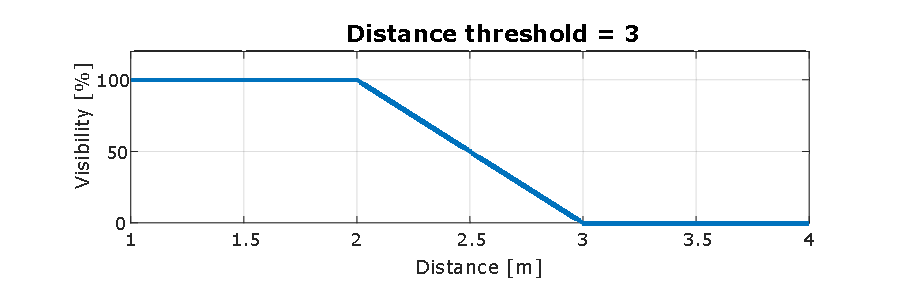
\includegraphics[width=\textwidth]{img/Simulation/falloff.eps}
        \caption{We consider a falloff distance of 1 m. Hence, for a threshold of 3 m, the tags closer to the camera than 2 m remain in the bag, tags at 2.5 meters have a 50~\% chance of being discarded, and all tags further away then 3 m are discarded.}
        \label{fig:falloff}
    \end{figure}
    
    \begin{figure}
        \centering
        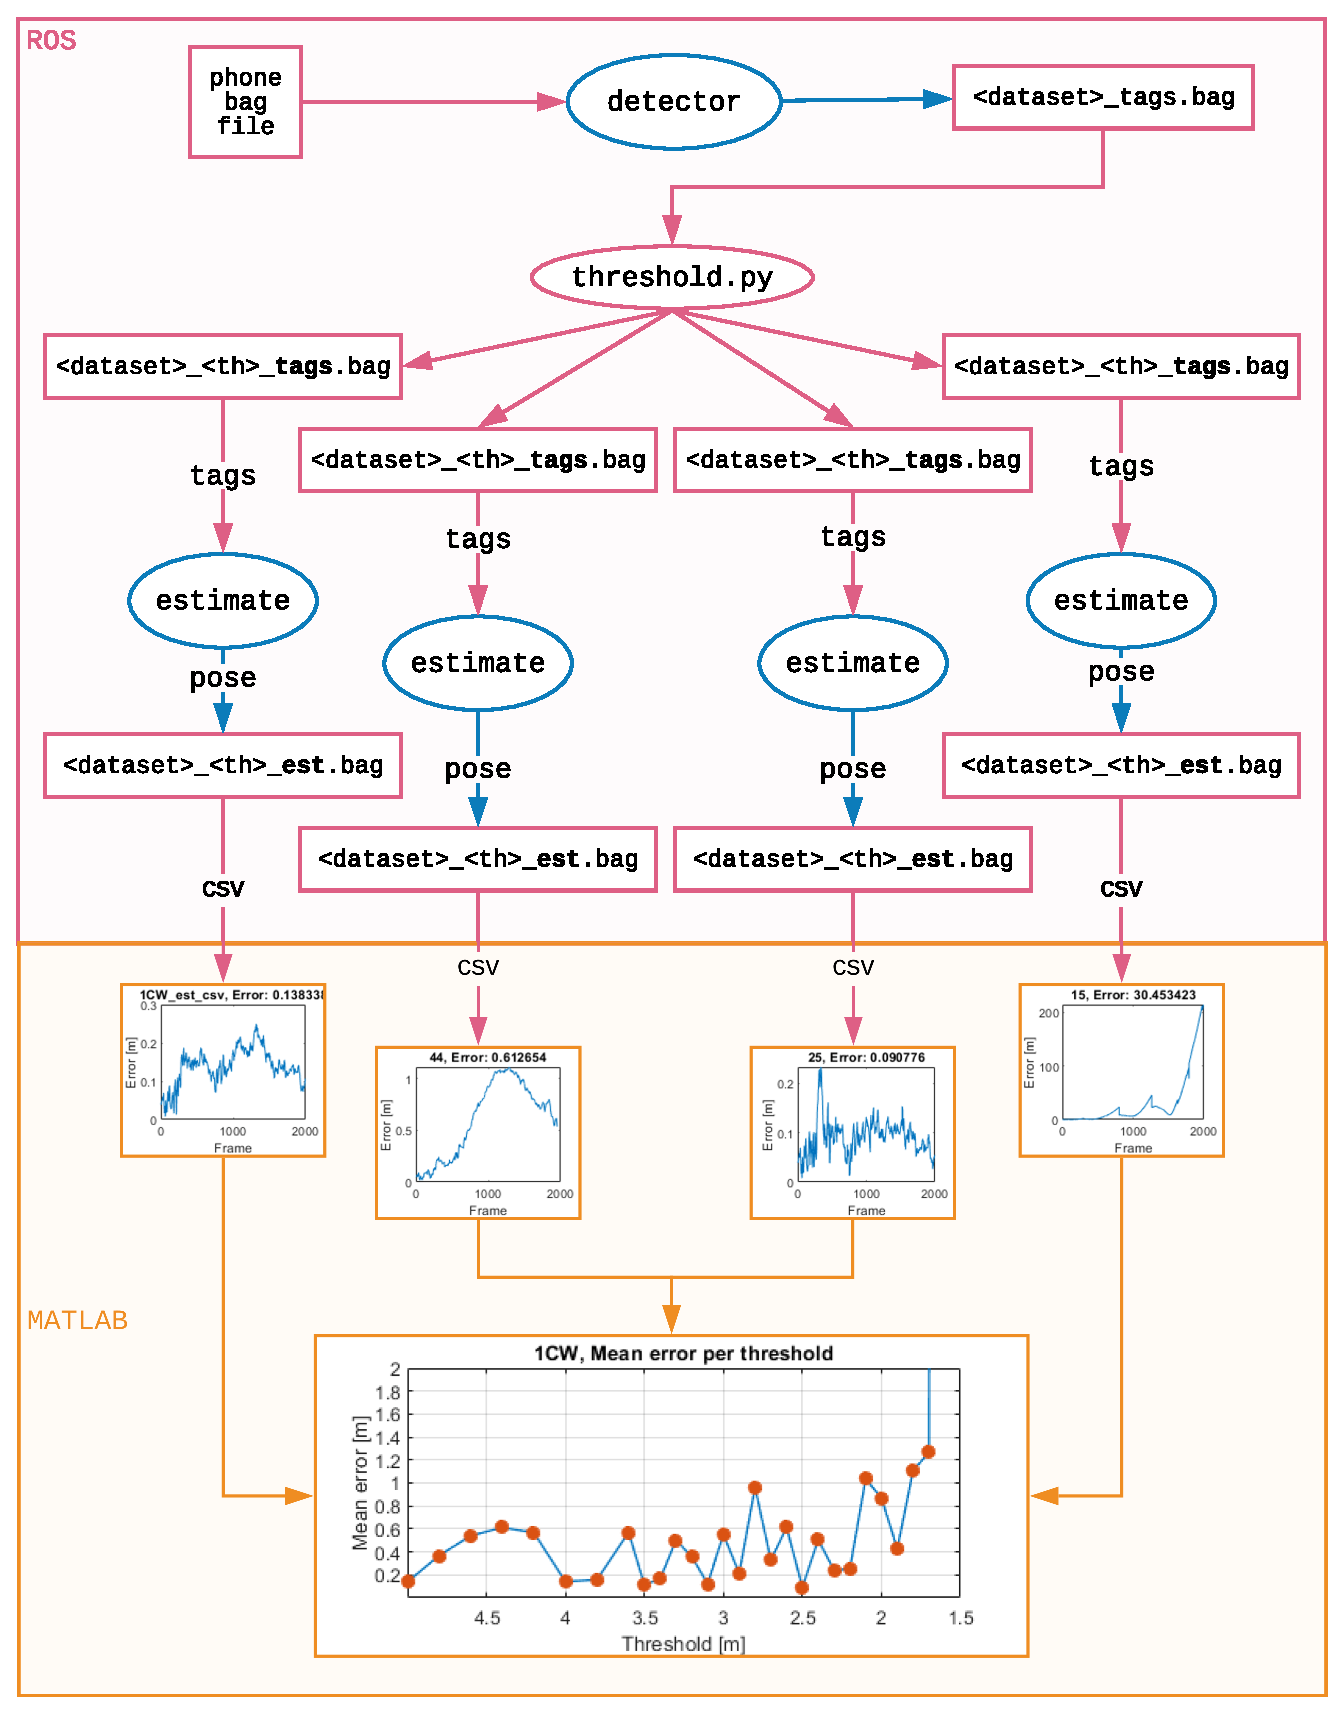
\includegraphics[width=.9\textwidth]{img/Simulation/workflow_sim.eps}
        \caption{Distance threshold simulation workflow. First, the detection is performed in full visibility conditions. Second, the markers are discarded according to a given threshold. Third, the leftover markers are sent to the estimator. Finally, MATLAB calculates the error per sample  for each threshold, which is input for the mean error per threshold plot.}
        \label{fig:workflow_sim}
    \end{figure}
    
    \subsection{Adding noise} \label{sec:noise}
    The second simulation assumes that there are floating particles in the water that bring noise into the image. We simulate this by corrupting the tag corner detection results by a random noise of a given variance. We make use of the fact that the EKF in RCARS uses the tag corner detections as measurement updates rather than directly the tag pose obtained by OpenCV. As a result of this holistic approach, we can improve the tracking by changing the \texttt{PixelStd} parameter in the \texttt{EKFsettings}.info file. The \texttt{PixelStd} parameter represents the pixel variance (the squared pixel standard deviation) of the tag corner detections.
    
    In full visibility, we use a pixel variance of 25 pixels. After adding noise to the corners, we raise this variance accordingly. For example, for an added noise with the variance of 100 pixels, we set the \texttt{PixelStd} parameter to 125.
    
    The workflow is similar to the thresholding. First, we obtain the full visibility \texttt{<dataset>\_tags.bag} file from the detector. Second, the \texttt{add\_noise.py} script adds zero-mean Gaussian noise with a given standard deviation to the tag detections. It uses the pseudo-random number generators Python module random\footnote{\url{https://docs.python.org/2/library/random.html}} with a seed of 250. Finally, a file named \texttt{<dataset>\_<stdDev>px\_<PixelStd>\_tags.bag} is output, which is then processed by the estimator to obtain the pose estimates in the file \texttt{<dataset>\_<stdDev>px\_<PixelStd>\_est.bag}.

\section{Evaluation method}
\label{sec:evaluation}
We evaluate the RCARS pose estimation accuracy of by computing the Euclidean distance between the 3D position of the smartphone estimated by RCARS and the position measured by the motion capture system (mocap). 
This section describes the evaluation method used in this thesis.
 
For data analysis and plotting, we use MATLAB\footnote{\url{https://www.mathworks.com/products/matlab.html}}. Thus, we wrote several MATLAB scripts to load the CSV files containing the pose estimates.
 
RCARS and the mocap are two independent systems that do not communicate with each other. To be able to compare them, their coordinate frames have to be aligned and their samples synchronized. When this is not done correctly, the evaluation results can be biased.

    \subsection{Coordinate frames alignment} \label{subsec:coord_align}
    \label{sec:coords}
    When aligning the coordinate frames, the task is to find a common coordinate frame for RCARS and the mocap. Both systems contain their own coordinate frames for the workspace, the tracking device, and the tag. In our method, we select a reference tag as the common coordinate frame, and transform the phone pose from the workspace frame to the local coordinate frame of the tag. Hence, the phone pose is in the local coordinate frame of the referene tag both for RCARS and the mocap.

    \subsection{Time synchronization}
    \label{sec:time_sync}
    After the poses from RCARS and mocap are aligned into a common coordinate frame, they have to be synchronized based on time. It is assumed that the mocap dataset is always longer than the phone recording because the recording on the mocap controller computer is started by the same person as the smartphone recording. Therefore, there is always a delay for a few seconds while the person moves to the initial position and starts recording on the smartphone. This is shown in \autoref{fig:delay}, where the recording on the smartphone was started 20 seconds after the mocap.
    
    \begin{figure}[b]
        \centering
        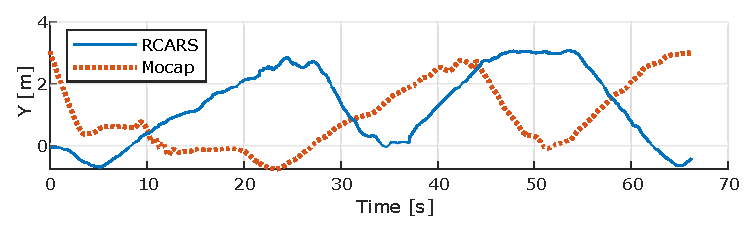
\includegraphics[width=.95\textwidth]{img/Simulation/Delay1.eps}
        \caption{The y-axes the mocap (blue) and RCARS (red) in a dataset, where the smartphone started recording 20 s after the motion capture.}
        \label{fig:delay}
    \end{figure}
    
    Since there is no grouping element in the CSV files of mocap and RCARS, we compute the cross-correlation between the positions in a given axis to find the count of samples that the mocap is ahead of RCARS. The choice of the axis depends on the range of motion in the dataset. From our tests, we prefer to use the x- or y-axis, since they are usually better estimated than the z-axis representing the height.

    Also, we found that the region for cross-correlation computing should not be the whole dataset but only the first few seconds. This is because we start the dataset recording with the camera pointing at the reference tag; therefore, even in the case when the filter is diverging, the error should be the smallest at the beginning and increase over time. Another case when it is necessary to take only the beginning of the dataset is when the RCARS estimates are delayed after the mocap measurements, as shown in \autoref{fig:delay}. If the cross-correlation determined the offset based on the whole dataset, the middle parts would be aligned and the beginning would be offset, which is against our assumption that the error is minimal at the beginning. By computing the cross-correlation only from the beginning of the dataset, we ensure that we find the initial alignment, not a global optimum.

    \begin{figure}[h]
        \centering
        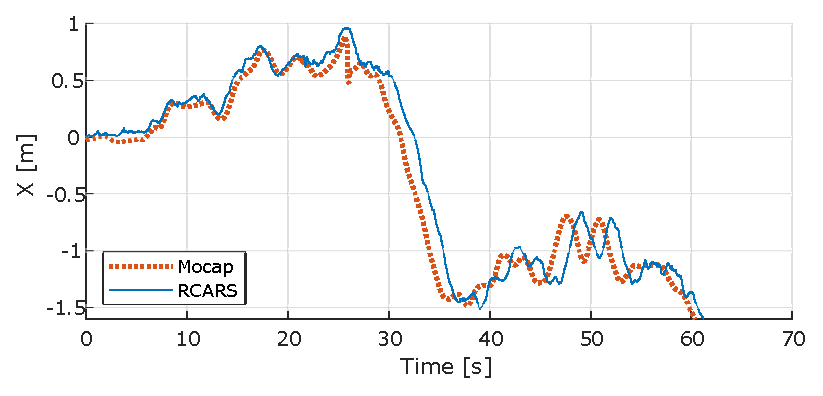
\includegraphics[width=\textwidth]{img/Simulation/Bgn.eps}
        \caption{The increasing delay between RCARS and mocap throughout the dataset. If the cross-correlation was computed on the whole dataset, it would be aligned based on the middle part. Thus, the cross-correlation takes into account only the first few seconds, depending on the dataset.}
        \label{fig:inc_delay}
    \end{figure}

\subsection{Error computation}
\label{sec:error}
    When the positions are aligned and synchronized, the error can be finally obtained by computing the Euclidean distance between the positions of mocap and RCARS at each time frame. The resulting plot is shown in \autoref{fig:error_frame}.
    
    \begin{figure}
        \centering
        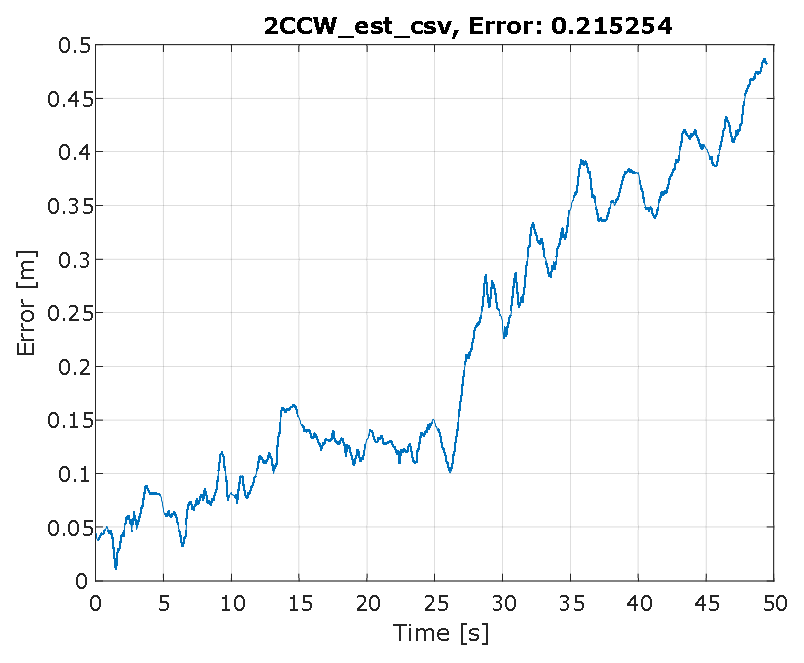
\includegraphics{img/Simulation/error.eps}
        \caption{The error per frame plot for the dataset \textit{2CCW}. The estimated pose is diverging from the ground truth, causing an increasing error over time.}
        \label{fig:error_frame}
    \end{figure}
    
    To evaluate the decreased visibility effects on the pose estimation, we run the estimator on many different thresholds and noise-corrupted detections, as shown in our simulation workflow in \autoref{fig:workflow_sim} on page \pageref{fig:workflow_sim}. These estimates are then joined in one plot showing the mean error per sample for a given threshold or noise standard deviation.

\chapter{Experiment}
Since it would be difficult to evaluate the effect of poor visibility conditions on the pose tracking directly underwater, we record the datasets in the controlled environment of a laboratory equipped with a motion capture system, serving as ground truth. We simulate the underwater conditions by post-processing the detection results, and produce estimates for each simulation. Finally, we calculate the error by comparing the obtained pose to ground truth and draw conclusions about the effect of our simulations on the pose tracking accuracy.

\section{Setup}
    \subsection{Laboratory}
    The experiments took place at the Human-Computer Interaction laboratory\footnote{\url{http://hci.fi.muni.cz/}} at the Faculty of Informatics, Masaryk University in Brno. The laboratory is equipped with a high-quality motion capture system from OptiTrack\footnote{\url{https://optitrack.com/products/prime-13w/}} that uses 16 ultra-wide cameras (Prime13W), offering high-precision and low-latency tracking with up to 240 FPS capture rate. Tracking of an object is realized by spherical retroreflective markers detected by the cameras. This system is controlled by the Motive software, which provides calibration, creating rigid bodies, and recording.
    
    \begin{figure}
        \centering
        \includegraphics[width=\textwidth]{img/Setup/HCIL.JPG}
        \caption{HCIL}
        \label{fig:hcil}
    \end{figure}
    
    Before recording the datasets, a new calibration was performed following the OptiTrack documentation\footnote{\url{https://v20.wiki.optitrack.com/index.php?title=Calibration}}, with exceptional results of the mean 3D error 0.673~mm. In our experiments, the average error per marker was 0.1~mm for rigid body of the static marker, and 0.4~mm for rigid body of the moving smartphone.

    \subsection{Markers}
    We used 27 pieces of AprilTag\footnote{\url{https://robot2016.mit.edu/sites/default/files/documents/project_apriltag36h11.pdf}} markers printed on A4 papers. As shown in \autoref{fig:hcil}, we placed the markers randomly throughout an area of 5.4 x 6.6 m in the laboratory. We attached them on horizontal, as well as vertical surfaces; while being careful not to bend their surface, which would affect the detections.

    To find the correct value for the \texttt{PxStd} parameter for the RCARS EKF in the conditions of our experiment, we built a static scene with the phone recording two markers at the distances of 1 m and 3 m for one minute. We then calculated the average standard deviation of the detected corners, resulting in 0.40811 pixels for the marker at 1 m and 0.44091 pixels for the marker at 3~m. However, the default \texttt{PxStd} parameter value is 25 pixels; but since we are recording in a higher resolution, we did not decrease this value and leave it on default.
    
    \subsection{Phone}
    The smartphone we used is the OnePlus 6 running on Android 9, equipped with a 16 MP f/1.7 wide-angle camera (25mm (wide), 1/2.6") and the BMI160\footnote{\url{https://www.bosch-sensortec.com/bst/products/all_products/bmi160}} IMU manufactured by Bosch Sensortec\footnote{\url{https://www.bosch-sensortec.com/}}.
    
    \subsection{Intrinsic calibration}
    We performed the camera calibration in the laboratory to assert equal lighting conditions than in the datasets recordings. We used the iMareCameraCalibration application, described in \autoref{subsec:input_data}, with a chessboard pattern of size 9 x 6 (the count of inner corners of the chessboard), and printed it on an A4 paper. The dimensions of one chessboard square were 25 x 25mm. The pattern, as well as the calibration images and coefficients, are provided in the attachments. 

    \subsection{Extrinsic calibration}
    Due to the extrinsic calibration, we have to know where the IMU is located in the device. We tried to figure out this location from the OnePlus 6 motherboard photos. Although it indicated possible locations, the exact one was not clear. 
    Therefore, we used the RCARS online extrinsic calibration. The obtained values are provided in the \texttt{EKFsettings.info} file in the attachments of this thesis. However, note that this estimate is still an approximation and may not reflect the true IMU location, thus the results may be affected by this error.
    
    \subsection{Phone rig}
    To track the phone pose with the motion capture system, we mounted the retroreflective markers tracked by the mocap cameras on the phone. Thus, we built a custom rig from skewers and rubber bands, shown in \autoref{fig:rig}. Following the marker placement recommendations from the documentation\footnote{\url{https://v20.wiki.optitrack.com/}}, we attached five spherical markers on the skewer edges asymmetrically to avoid congruency. This phone rig has proved to be robust enough against deflection, and, with the proper holding of the device, the rig is trackable by the motion capture system throughout the whole dataset with minimal detection loss.
    
    When a rigid body of this rig is created in Motive, its pivot point is at its geometric center. Thus, to translate the pivot point to the camera location, we measure the distance from the camera lens to the geometric center of the phone, and translate the pivot point in Motive accordingly.
    
    \begin{figure}
        \centering
        \includegraphics[width=\textwidth]{img/Setup/Rig.png}
        \caption{The dimensions of the phone rig mounted on the OnePlus 6. The mocap retroreflective markers are placed asymmetrically to avoid ambiguity. To track the pose of the camera instead of the geometrical center of the rig, the rigid body pivot point is translated by 4.75~cm in Motive.}
        \label{fig:rig}
    \end{figure}

    \subsection{Motion capture to filter estimation}
    As proposed in \autoref{subsec:coord_align} on page \pageref{subsec:coord_align}, the poses have to be aligned according to a common origin to be able to compare the poses measured by the motion capture and the filter. In this case, the origin is set to be the AprilTag with id 1.
    
    The origin of the tag coordinate frame in OpenCV is in its geometrical center. Similarly, when a rigid body is created in Motive, its pivot point is in its geometric center. Thus, the tracking of the tag by the mocap is achieved by placing the retroreflective markers onto the four tag corners (see \autoref{fig:tagMocap}), and consequently creating a new rigid body in Motive. Hence, we ensure that the origin of the marker pose is the same for both RCARS and the motion capture.
    
    \begin{figure}
        \centering
        \includegraphics[width=\textwidth]{img/Setup/tagMocap.JPG}
        \caption{The mocap retroreflective markers are placed onto the corners of the reference tag so that the pivot point of the new rigid body is in the geometrical center of the tag. Note that the markers cannot be placed directly onto the edges of the black square, because it would disable the OpenCV detection. Neither could the markers be placed onto the edges of the A4 paper, because the black square was offset by 1.1 cm to the top of the paper, so the pivot would not be in the center of the black square.}
        \label{fig:tagMocap}
    \end{figure}
    
    \subsection{Recording}
    For recording the datasets on the smartphone, we used the iMareCameraRecorder developed by Jan Čejka. A recording contains the accelerometer, the gyroscope, and the magnetometer measurements, and the camera images with their corresponding timestamps. Note that the camera frames and the IMU samples are not synchronized as in the case of the specialized VI-Sensor, which may negatively affect the performance of the estimator.
    
    The application contains a configuration file for setting the image resolution and sampling rates. In the experiments, we used the image resolution of 1280 x 720 pixels captured at 30 frames per second, and the IMU sampling rates of 200Hz for the gyroscope and 400Hz for the accelerometer. However, due to the RCARS input requirements, the \texttt{phone\_to\_bag.py} downsamples the accelerometer to match the sampling rate of the gyroscope.
	
	\subsection{Computer}
	To run RCARS for estimation and MATLAB for evaluation, we primarily use the Lenovo Z580 laptop with Intel Core i7-3612QM 2.10GHz CPU and 8 GB RAM. In addition, due to large file sizes and high computational cost of the detection and estimation, we use a workstation in our laboratory with Intel Core i7-8700 3.20GHz CPU and 32 GB RAM.
	
	\subsection{RCARS}
	To run RCARS, we downloaded a Ubuntu 14.04 LTS virtual machine accessible on Nootrix.com\footnote{\url{https://nootrix.com/diy-tutos/ros-indigo-virtual-machine/}}, which has already preinstalled ROS Indigo and ROS tools. Then, we installed RCARS according to the instructions in the project's repository\footnote{\url{https://bitbucket.org/adrlab/rcars/wiki/Home}}.
	
    Since we are recording our datasets in HD resolution, working with a large number of markers, and running RCARS on a virtual machine, we run the detector first, save the detection results, and then run the estimator separately. Moreover, we play all bag files at slower speeds to lower the computational demands and ensure the best detection and estimation possible.

\section{Datasets}
In order to execute the simulations described in \autoref{sec:simulating} on page \pageref{sec:simulating}, we recorded three different datasets: \textit{1CW}, \textit{2CCW}, and \textit{3RAND}. Figures \ref{fig:1CW}, \ref{fig:2CCW}, and \ref{fig:3RAND} show the 3D trajectories of RCARS and mocap, as well as the error per frame plots for each dataset. This section introduces the datasets by the full visibility pose estimates.

In the dataset \textit{1CW}, we walk slowly one time around the room clockwise. We are avoiding rapid changes in movement or orientation because our goal is to test the filter robustness against a low number of markers, not against fast motions. However, shake still occurs due to walking. This dataset is 67~s long and has the lowest error out of the three: in average 13~cm/frame.

In the dataset \textit{2CCW}, we again walk slowly around the room, but this time in the counter-clockwise direction to test if the direction of the movement in our setup affects the pose estimation. However, a large outlier occurred in the half of the dataset, so we decided to remove it by trimming the dataset to the half of its original length. Hence, the dataset is 50~s long and the error accumulates over time to up to 49~cm at the end. The average error is 22~cm/frame.

Finally, the dataset \textit{3RAND} contains random trajectory movement with several fast motions that, this time, also test the filter robustness against rapid motions. This kind of incautions use occurs when the system is used by inexperienced users, not aware of the importance of minimizing motion blur and shake. This dataset is trimmed to 66~s and has the largest average error: 32~cm/frame. In contrast with \textit{2CCW}, the error does not accumulate over time; instead, it jumps at a certain point (due to a rapid movement) and then converges to its true value, but then again an outlier occurs, and the error rises.

\begin{figure}[p]
    \centering
    \begin{minipage}{.49\textwidth}
        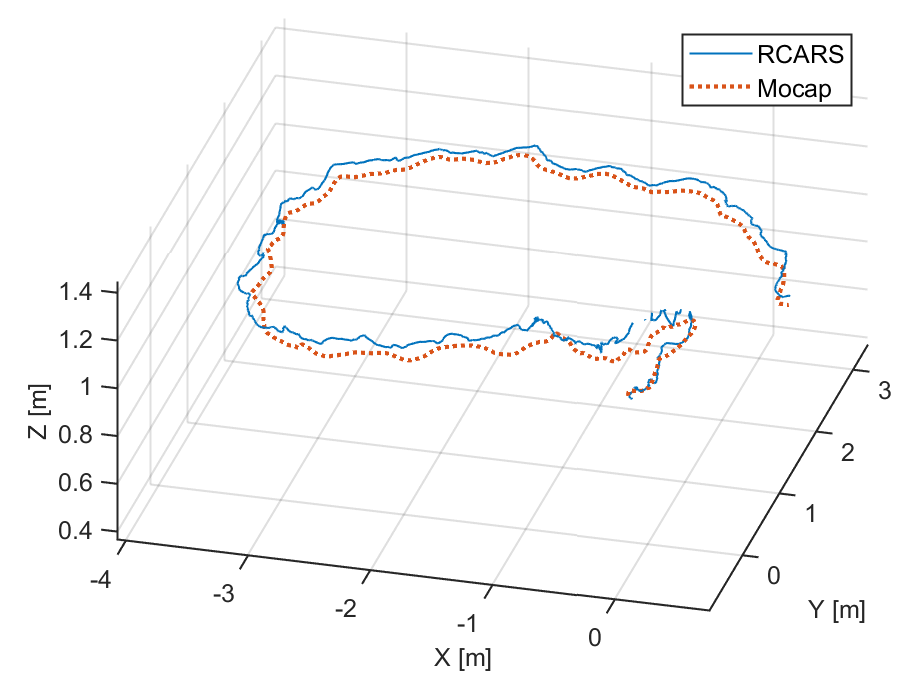
\includegraphics[width=\textwidth]{img/Experiments/1CW/3D.eps}
    \end{minipage}
    \begin{minipage}{.49\textwidth}
        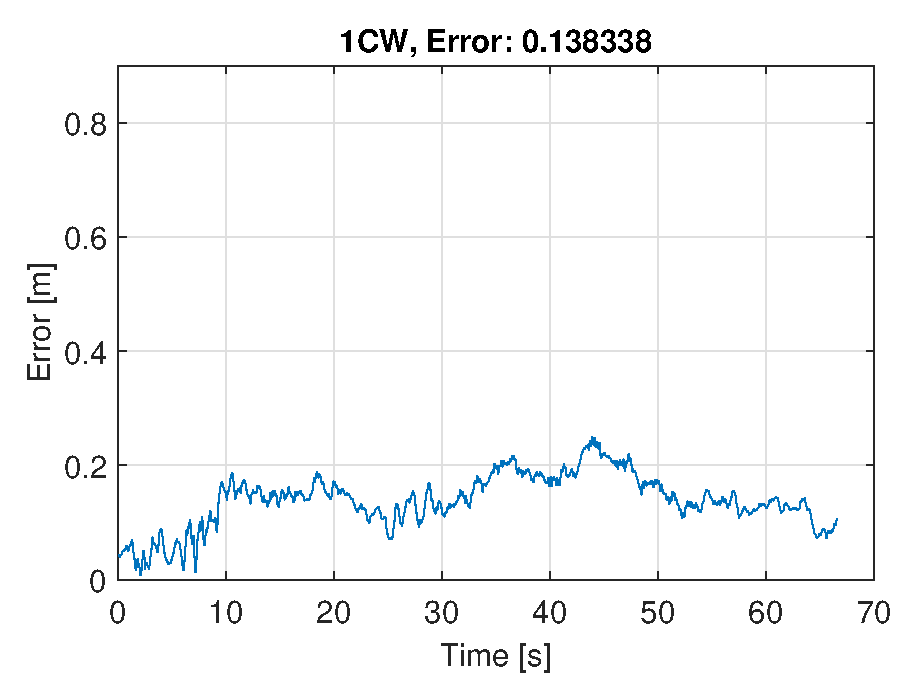
\includegraphics[width=\textwidth]{img/Experiments/1CW/Err.eps}
    \end{minipage}
    \caption{1CW}
    \label{fig:1CW}
\end{figure}

\begin{figure}[p]
    \centering
    \begin{minipage}{.49\textwidth}
        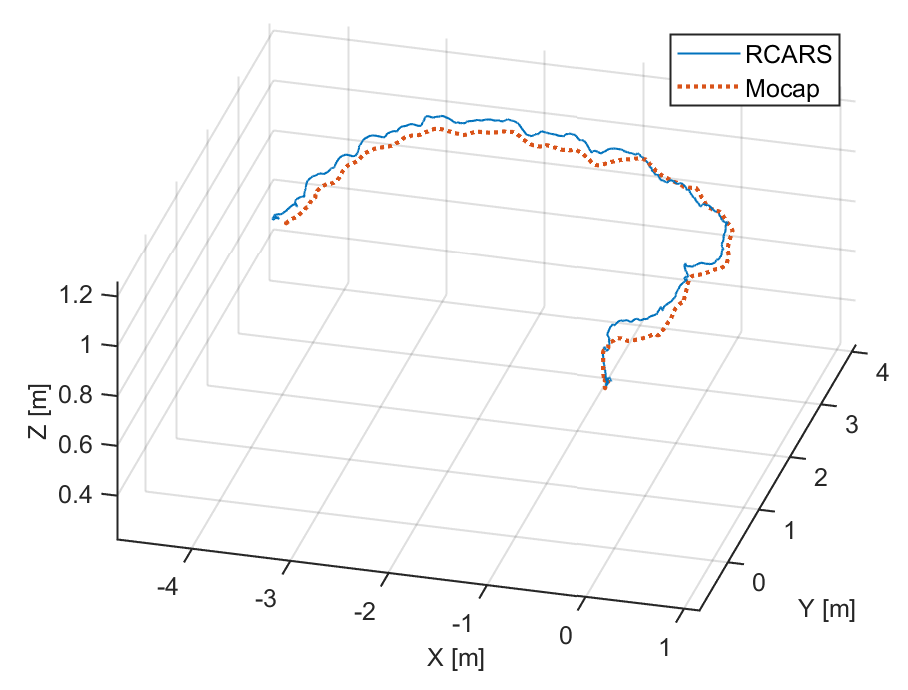
\includegraphics[width=\textwidth]{img/Experiments/2CCW/3D.eps}
    \end{minipage}
    \begin{minipage}{.49\textwidth}
        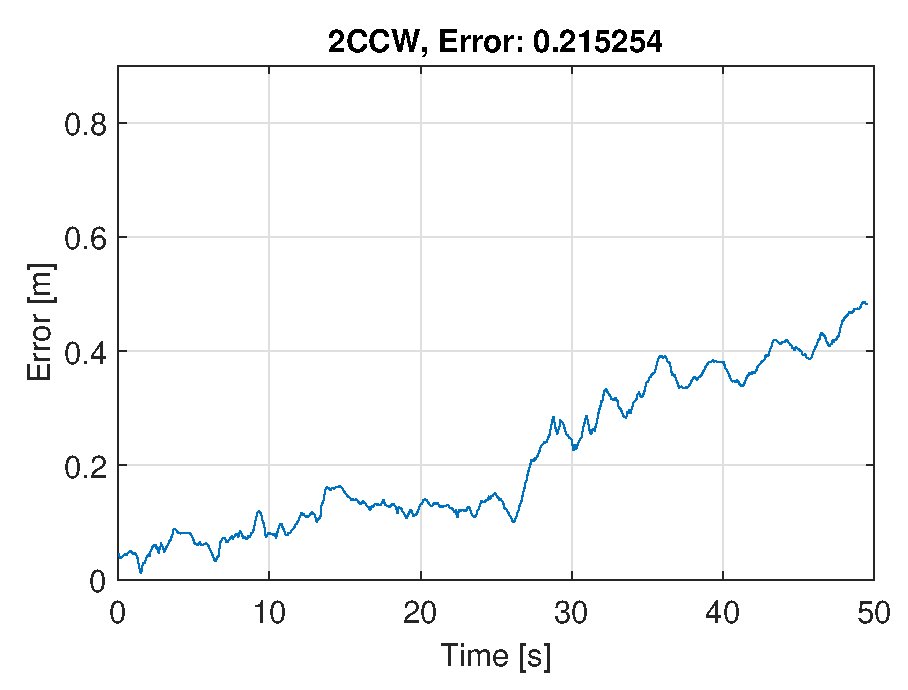
\includegraphics[width=\textwidth]{img/Experiments/2CCW/Err.eps}
    \end{minipage}
    \caption{2CCW}
    \label{fig:2CCW}
\end{figure}

\begin{figure}[p]
    \centering
    \begin{minipage}{.49\textwidth}
        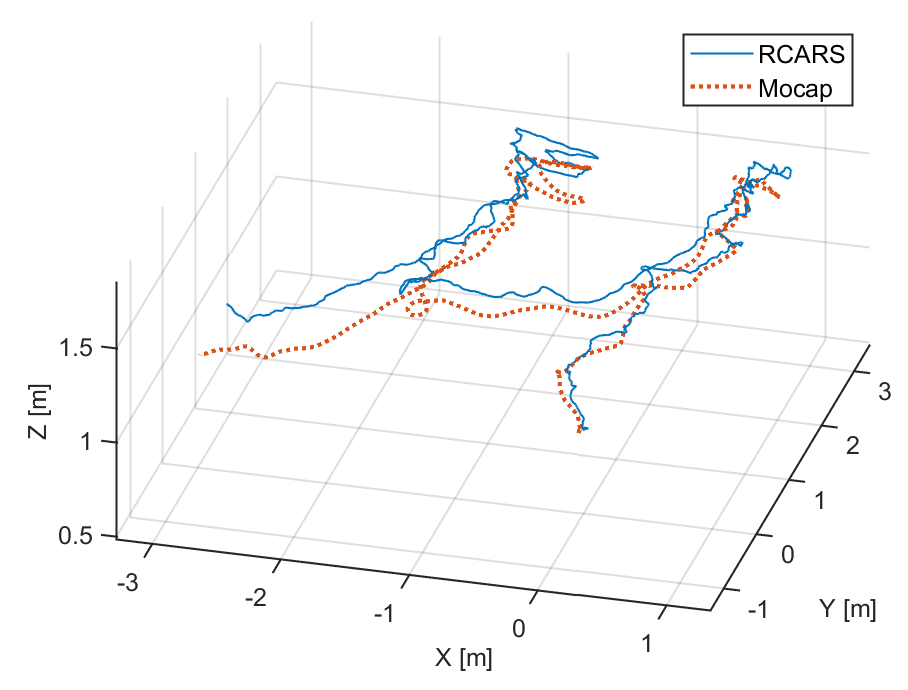
\includegraphics[width=\textwidth]{img/Experiments/3RAND/3D.eps}
    \end{minipage}
    \begin{minipage}{.49\textwidth}
        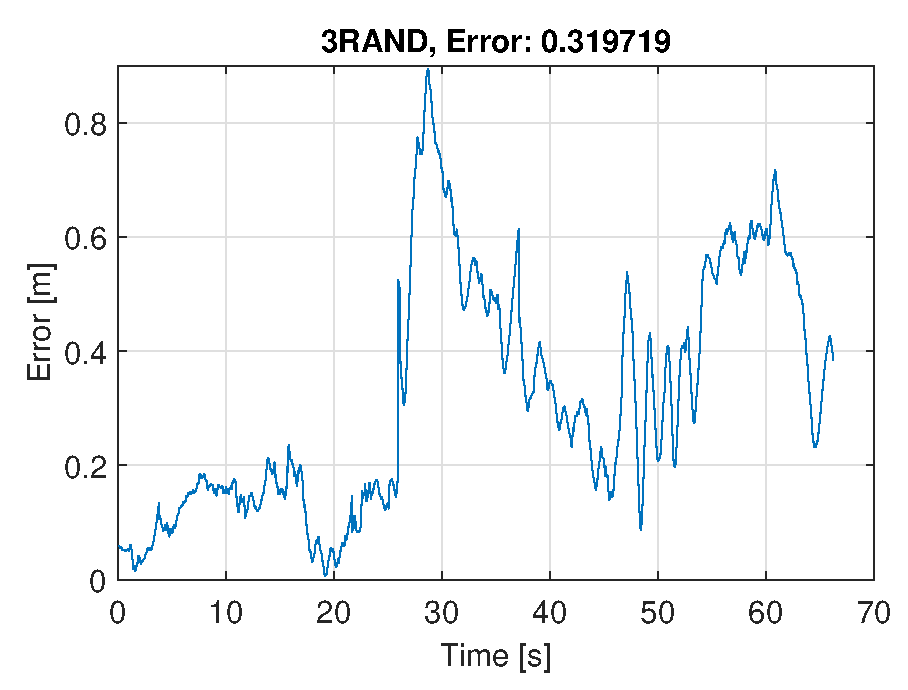
\includegraphics[width=\textwidth]{img/Experiments/3RAND/Err.eps}
    \end{minipage}
    \caption{3RAND}
    \label{fig:3RAND}
\end{figure}

\section{Results}
    
    \subsection{Distance threshold}
    We estimated a number of thresholds in the interval from 1.5 to 5~m, focusing primarily on the thresholds below 3~m; thus, the thresholds are denser in the interval from 1.5 to 3~m, with an offset of 10~cm, while the more distant thresholds than 3 meters are estimated every 20~cm. This subsection gives commentary to the results.
    
    \subsubsection{Same errors, different plots}
    By decreasing the distance threshold, the count of detected images also decreases. When there is no image detected, the estimations are based only on the inertial measurements, and therefore the filter starts drifting away. This is shown in \autoref{fig:07_drift} for the dataset \textit{2CCW} --- even though the error at 1.8~m is lower than at 2.4~m by almost 5~cm, there is a significant difference in the estimation process, and thus also in the AR experience. While at 2.4~m the error accumulates gradually, at 1.8~m the filter starts diverging several times and jumps back near its true position when a marker is detected.
    
    \begin{figure}
        \centering
        \includegraphics[width=\textwidth]{img/07_drift.png}
        \caption{Dataset \textit{2CCW} estimations at 2.3 m on the left, and 1.8 m on the right. Note that even though the mean error is lower at 1.8 m, the pose is drifting away in the highlighted areas; while the estimation at 2.3 m contains no drift.}
        \label{fig:07_drift}
    \end{figure}
    
    \subsubsection{Mean error per threshold}
    \autoref{fig:mean_error__per_threshold} shows the mean error per threshold for each dataset. Although we expected that with decreasing threshold, the error would gradually rise, the results do not fully follow this inverse proportionality.
    
    \begin{figure}
        \centering
        \includegraphics[width=\textwidth]{img/thresholds.png}
        \caption{TODO: Horizontally. Mean error per threshold plots for each dataset.}
        \label{fig:mean_error__per_threshold}
    \end{figure}
    
    Instead, every dataset contains a threshold below 3~m where an outlier occurs, i.e., where the error significantly lower than the error in the neighboring thresholds. What is more, the errors of these outliers are at times as low or even lower than in 100~\% visibility, resulting in the peaks shown in FigX. For example, in the case of the dataset 1CW, where the mean error per sample at full visibility is 14~cm, but at 2.5~m is only 9~cm. For the dataset \textit{2CCW}, this occurs at the threshold of 2.2~m, with a 1~cm lower error than in the full visibility estimate.
    
    To verify that the peaks are not caused by the detector or estimator running too fast, we executed both the detection and estimation repeatedly on slower speeds and different computers. However, the results still stay the same.
    
    \subsubsection{Minimum threshold}
    With the threshold below 2~m, the estimation in all datasets often diverges by tens of meters. \autoref{fig:low_thresholds} contains plots showing the errors per frame in low thresholds for all datasets.
    
    \begin{figure}
        \centering
        \includegraphics[width=\textwidth]{img/low_thresholds.png}
        \caption{Errors per frame in low thresholds}
        \label{fig:low_thresholds}
    \end{figure}
    
    We are interested in finding a minimum threshold where the tracking still reaches similar accuracy to the tracking in higher visibility. If the minimum threshold is taken from the mean error per threshold in \autoref{fig:mean_error__per_threshold}, \autoref{tab:edge_thresholds} shows the result, along with the average number of tags detected per frame in the estimation. The results indicate that at the visibility below 2.2 m, frequent marker detection losses occur, which causes the pose to diverge. This drift also happens when there is no marker detected in more than one image out of four.
    
    \begin{center}
        \begin{table}
            \begin{tabular}{l|lll}
                \toprule
                & 1CW & 2CCW & 3RAND \\
                \midrule
                Threshold (m) & 2.2 & 2.2 & 2.5 \\
                Average detected tags & 0.7864 & 0.7453 & 0.6071 \\
                \bottomrule
            \end{tabular}
            \caption{Edge distance thresholds for datasets}
            \label{tab:edge_thresholds}
        \end{table}
    \end{center}
    
    \subsubsection{Discussion}
	The results show that too many markers in the image, or detecting also distant markers when already closer ones are detected, does not improve the estimation accuracy. What is more, as in the case of dataset 3RAND shown in Fig.X, the distant markers can even decrease the accuracy. Thus, redundant distant markers may be discarded to reduce the map size of the estimation problem and lower the computational demands.
	
	Answering the question of why the spikes in \autoref{fig:mean_error__per_threshold}, is not in the scope of this thesis and is subject to future research. However, we assume that one of the reasons why the estimates in lower visibility are less accurate than in higher visibility is that the distant markers bring false information into the estimation.
	
	For example, we assume that the peak in \textit{3RAND} at 3.6~m occurred as follows. While for higher thresholds there were more distant markers that contributed to the tracking well, at 3.6~m they are not detected anymore, but there are still distant markers that may bring false information due to their placement or the device movement, which harms the estimation. By lowering the threshold to 3.4~m, these tags are discarded, thus, not bringing false information into the estimation. 
	
	We also assume that this interference by distant markers is occurring periodically in the rest of the dataset 3RAND, as well as in 1CW. We suppose that it could be controlled by adjusting the EKF parameters \texttt{PixelStd} and \texttt{MahalanobisTh}. The pixel standard deviation parameter sets the impact of the tag detection on the estimation. Although increasing it would cause fewer outliers, it would be for the price of a lower accuracy. On the other hand, lowering the Mahalanobis threshold would result in more frequent outliers; thus, the tag poses would be more frequently reset, and the system would have a higher chance of recovery. 
    
    \subsection{Added noise}
    We added zero-mean Gaussian noise to the tag corner detections with the standard deviations of 2, 5, 8, 10, 15, and 20 pixels, and respectively raised the \texttt{PxStd} parameter, representing the squared pixel standard deviation in the EKF estimation. Since the value of this parameter in full visibility is 25 pixels, after corrupting the detection results with the noise of standard deviation $\sigma$, the resulting value for the PxStd is $25 + \sigma^2$. \autoref{fig:noise} shows the output of this simulation in a mean error per noise standard deviation plot for every dataset.

    \begin{figure}
        \centering
        \includegraphics[width=\textwidth]{img/noise.png}
        \caption{TODO: Horizontal pltos. Errors per noise standard deviation}
        \label{fig:noise}
    \end{figure}
    
    The results are similar for the datasets \textit{2CCW} and \textit{3RAND}. By adding noise of even 2~pixels, the mean error per sample rises from 22~cm to 65~cm in \textit{2CCW}, and from 31~cm to 65~cm in \textit{3RAND}. After continually increasing the amount of noise, the mean errors in \textit{3RAND} stay on 65~cm +- 1~cm to up to 15~pixels, while the mean errors in \textit{2CCW} stay on 65~cm +- 5~cm up to 10~pixels, and at 15~pixels, the error rises to 80~cm per sample. However, with the noise standard deviation of 20~pixels, the mean error significantly decreases in both datasets.
    
    In contrast, the mean errors in \textit{1CW} rise and drop randomly, ranging from 13~cm at full visibility up to 109~cm at 8~pixels.
    
    \subsubsection{Discussion}
    The datasets \textit{2CCW} and \textit{3RAND} confirm that by taking into account the pixel variance in the EKF estimation, the estimation accuracy is kept on the same level, or may even increase due to the large variance parameter. 
 
    A subject of future work can be determining the PxStd value for the device, as we left it on the default 25~pixels, but it has a considerable influence on the estimation accuracy.
    
    
\chapter{Conclusion}
In this thesis, we analyzed the underwater challenges of AR systems that are based on hybrid pose tracking and use Kalman filters for sensor fusion. We first chose a solution that meets our requirements, RCARS, and utilized it for the use with smartphone recordings. Using this system, we evaluated the effect of decreased visibility conditions simulated in a laboratory equipped with a motion capture system as ground truth.

We simulated the underwater conditions by discarding markers according to their distance from the camera and by corrupting the detected corners by adding artificial noise to simulate water turbidity. 

The results on our datasets show that the pose estimation accuracy of the system in 2.2~m visibility is on the same level as in 3, 4, or even 5~m visibility. Thus, we conclude that the system does not need a high number of markers to produce accurate pose estimates. Instead, the number of detected markers can be even decreased to reduce computational complexity and, thus, improve the estimation speed.

From our experiments, we learned that for EKF-based systems, proper configuration is critical for satisfactory pose estimation. The experiment of adding noise to the detection showed that when the correct pixel standard deviation parameter is provided, the system can produce precise pose estimates even in a very turbid environment. However, these parameters are device dependent; finding them is not trivial and requires some experience. 

\section{Future work}
Since even a low number of markers is enough for quality estimates, future work could concentrate on analyzing datasets with sparsely placed markers. For this purpose, the RCARS visualization package is helpful, because it provides live pose estimation in a 3D workspace and an image preview that contains both the marker detections and the corresponding estimations. This tool can also be used for finding the appropriate EKF parameters for the device to minimize the bias caused by improper EKF configuration. 

Furthermore, other devices could be used for testing, since the system is also affected by the field of view, the autofocusing system of the camera, and the camera and IMU synchronization.
The intrinsic camera calibration depends on the field of view, which depends on the focusing distance. Thus, the calibration parameters can be obtained only for one focusing distance. However, when the camera's autofocus is enabled, the focusing distance changes throughout the dataset, causing the calibration parameters to be outdated. This problem can be tackled by saving the calibration parameters for various focusing distances and interchanging between them online during the detection.
In the video recordings of our datasets, \textit{focus breathing} of the autofocusing system occurred, which brings the tags temporarily out of focus, leading to detection loss. The “focus breathing” can be solved either by using a smartphone with a better autofocusing system or by disabling the autofocus and setting the focus to a proper distance. However, due to poor lighting conditions underwater, the cameras use large apertures leading to a shallower depth of field in the image, which increases the amount of blur in the background and the foreground; thus, possibly harming detection.
 
Another possible source of bias in our experiment is the pose alignment between RCARS and the motion capture system. Thus, instead of using the absolute alignment into one coordinate frame, one could compare their relative measures, such as the angular velocity or the total distance covered.
 
The future work could also concentrate on the development of marker-less SLAM based solutions that detect natural features instead of markers. However, this may lead to higher computational demands on the mobile device in both the detection and the estimation. Moreover, simulating underwater conditions for such systems is a whole new challenge.


\printbibliography[heading=bibintoc] %% Print the bibliography.
\end{document}